\documentclass[a4paper, 11pt]{article}

	\usepackage[utf8]{inputenc}
	\usepackage[T1]{fontenc}
	\usepackage[french]{babel}
	\usepackage{amsmath}
	\usepackage{graphicx}

	\usepackage{graphicx}

    \title{HAUMTinsel 2015}
    \author{HAUM}
	\date{Novembre 2015}


\begin{document}
	\maketitle

\section{Dispositif}

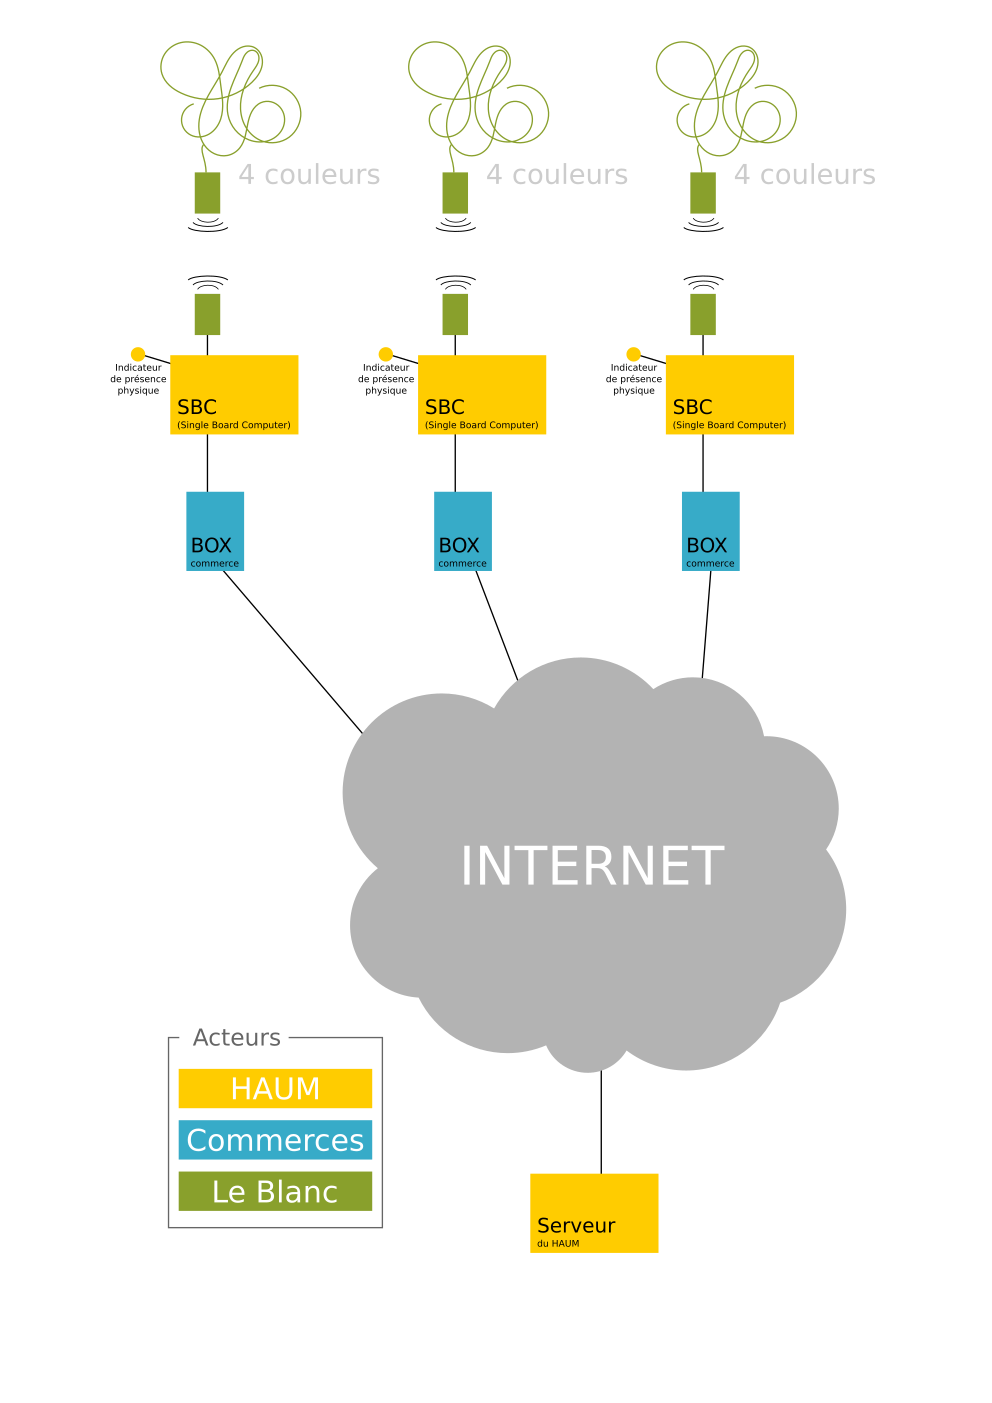
\includegraphics[width=12cm]{general_architecture.png}

Dans l'ordre il y a :

\begin{itemize}
	\item Indicateur de présence physique
	\item Bandes RGB/installation à poser (fourni par LeBlanc)
	\item Connexion RF entre la SBC et le décor (fourni par LeBlanc)
	\item SBC (RaspberryPi du HAUM + prêts)
	\item Connexion Internet (fourni par le commerce hôte)
	\item Serveur (dédié d'un des membres du HAUM)
	\item Explications dans la rue (encart)
\end{itemize}

\section{Côté Serveur}

Un sous-domaine est mis à disposition (typiquement \texttt{fetes15.haum.org}) et les URLs courtes sont crées pour
simplifier le travail aux utilisateurs.

Un jeu différent est proposé pour chaque point, l'idée de départ se basant sur 3 points, voilà trois exemple de jeux :

\begin{itemize}
	\item Simon Say 3x3
	\item Hit the Santa Claus ! (voir jeu de l'an dernier)
	\item Tape la taupe avec 2 taupes en même temps
\end{itemize}

La difficulté des jeux doit être variable pour s'assurer qu'il y a toujours du challenge.

Les équipes sont formées automatiquement à partir d'un pseudo mappé vers les couleurs.

Le client se connecte via un navigateur web, il est donc possible de pousser des notifications aux utilisateurs.

\subsection{Comment gagner des points}

Quand la partie est gagnée, on ajoute des points aux scores de l'équipe.

Pour rendre le jeu plus intéressant, les points diminuent avec le temps (il faudra peut être prévoir deux taux de
diminution pour le jour/nuit).

L'affichage des scores en ligne est indispensable pour la communication :

\begin{itemize}
	\item carte visuelle
	\item twitter
	\item graphe (avec retard)
	\item facebook
\end{itemize}

\section{Incentives}


\begin{itemize}
	\item Coupons limités chez les commerçants (distribués au changement de couleur d'un point)
	\item 3 Points de la même couleur $\Rightarrow$ suggestion de rencontre
\end{itemize}

\end{document}

